% Reproducible manuscript source — target: Explorations in Economic History
% Generated by create_manuscript_latex.py
\documentclass[pdflatex,sn-basic]{sn-jnl}

\usepackage{graphicx}%
\usepackage{multirow}%
\usepackage{amsmath,amssymb,amsfonts}%
\usepackage{amsthm}%
\usepackage{mathrsfs}%
\usepackage[title]{appendix}%
\usepackage{xcolor}%
\usepackage{textcomp}%
\usepackage{manyfoot}%
\usepackage{booktabs}%
\usepackage{algorithm}%
\usepackage{algorithmicx}%
\usepackage{algpseudocode}%
\usepackage{listings}%
\usepackage{hyperref}
\usepackage[T1]{fontenc}

\theoremstyle{thmstyleone}%
\newtheorem{theorem}{Theorem}%
\newtheorem{proposition}[theorem]{Proposition}%
\theoremstyle{thmstyletwo}%
\newtheorem{example}{Example}%
\newtheorem{remark}{Remark}%
\theoremstyle{thmstylethree}%
\newtheorem{definition}{Definition}%

\raggedbottom

\begin{document}

\title[Network Exclusion and State Collapse]{Network Exclusion and State Collapse: From Maritime Isolation to Technological Access Denial in the Long Run of History}

\author*[1]{\fnm{Author} \sur{Name}}\email{author@example.com}

\affil*[1]{\orgdiv{Department}, \orgname{University}, \orgaddress{\street{Street}, \city{City}, \postcode{00000}, \state{State}, \country{Country}}}

\abstract{
Why do some states collapse while others endure? This exploratory study proposes that structural exclusion from the dominant technological network of an era---not merely deliberate trade closure---is a candidate correlate of state vulnerability, with technology-flow disruption proposed as one possible explanation for divergence between connected and excluded polities. Using a comparative dataset of 96 historical polities spanning antiquity to the present, assembled as an AI-assisted exploratory dataset rather than a public-data measurement dataset, we distinguish between policy-driven isolation (e.g., Ming \emph{haijin}, Tokugawa \emph{sakoku}) and what we term `technical network exclusion': involuntary disconnection from prevailing exchange networks due to geographic or technological constraints. Policy-based closure can reduce without eliminating technology transfer (e.g., \emph{rangaku} via Dejima under \emph{sakoku}), whereas technical exclusion is coded as more severe involuntary disconnection. Across a post hoc reclassification of 7 technically excluded polities, the one-sided Fisher exact p-value for closure and conquest changes from 0.187 to 0.020; all 7 were coded as eventually conquered. Within these exploratory codings, multivariate logistic regression shows the largest conditional associations for external threat and institutional quality, while the stock--flow odds ratio (OR $= 1.774$) remains stable across all scenarios. We present the underlying mechanism---technology flow disruption leading to an accumulating civilization-level gap---as a hypothesis beyond maritime isolation. As the dominant network shifts from sea lanes to semiconductors, artificial intelligence, and advanced robotics, states structurally excluded from these technological platforms may face analogous vulnerabilities.
}

\keywords{network exclusion, economic history, technology flow disruption, state collapse, technological access, sensitivity analysis}

\maketitle

\section{Introduction}\label{sec:intro}

Every era has a dominant network---a prevailing infrastructure of exchange through which states access trade, technology, and strategic information. In antiquity, it was the Mediterranean sea lanes and the Silk Road caravan routes. In the age of sail, it was transoceanic maritime commerce. In the industrial age, it was railroad-linked factory systems and colonial supply chains. Today, it is the digital and semiconductor ecosystem. A recurring pattern in global history is that states excluded from the dominant network of their era---whether by choice or by circumstance---face elevated risks of decline and conquest \citep{Kennedy1987, FindlayORourke2007}.

The existing literature offers two broad explanations for why states fail. One emphasizes internal dynamics: \citet{Tainter1988} argued that complex societies collapse when the marginal returns to increasing complexity decline, and \citet{AcemogluRobinson2012} showed that extractive institutions---those that concentrate power and discourage innovation---undermine long-run prosperity. The other emphasizes external connectivity: trade openness, technology diffusion, and the consequences of isolation \citep{FindlayORourke2007, Mokyr2002}. Our contribution lies at the intersection. We examine whether disconnection from the dominant exchange network is associated with institutional quality and technological capacity---the factors that the internal-dynamics literature identifies as proximate explanations of collapse.

The literature on trade and isolation has overwhelmingly focused on deliberate closure: the maritime prohibitions (\emph{haijin}) of Ming China, the \emph{sakoku} decree of Tokugawa Japan, the autarkic blocs of the Cold War. Deliberate closure is analytically convenient because it represents a policy choice with an identifiable agent. Yet this focus on intentional closure overlooks a logically prior question: what happens to polities that never had the option of connecting to the dominant network in the first place? The Khmer Empire at Angkor, the Kievan Rus' principality, or the Timurid dynasty were not isolated because their rulers chose closure; they were isolated because the dominant exchange networks of their era did not reach them. If these polities exhibit the same elevated conquest risk as deliberately closed ones, then the pattern would be consistent with disconnection, rather than the policy decision alone, as a candidate explanation.

We hypothesize that technology flow is a relevant channel. Maritime trade was never merely an exchange of goods; it was the primary vehicle through which military techniques, navigation methods, metallurgy, and institutional innovations diffused across polities \citep{Pomeranz2000, Mokyr2002}. Deliberate closure, such as \emph{sakoku}, restricted but did not eliminate this flow---Tokugawa Japan maintained a narrow conduit of Western scientific knowledge (\emph{rangaku}) through the Dutch trading post at Dejima. Technical exclusion, by contrast, is hypothesized to restrict a broader set of channels. A possible result is a cumulative technology gap: over generations, excluded polities may fall behind the technological frontier, and when contact with a more advanced civilization eventually occurred---often through military confrontation---the gap may have increased vulnerability. This is, in essence, a quantitative restatement of a long-recognized pattern: when civilizations at markedly different technological levels collide, the less advanced one may face elevated vulnerability \citep{Diamond1997}.

This paper makes three contributions. First, we construct a comparative historical dataset of 96 polities spanning six eras (ancient, medieval, early modern, modern, twentieth century, and contemporary) and classify each along two dimensions: its predominant resource base---stock-oriented (accumulated assets such as human capital, institutions, and natural resources) versus flow-oriented (trade, military projection, and diplomatic engagement)---and its degree of closure from international networks. Second, we introduce the concept of `technical network exclusion,' defined as the involuntary disconnection of a polity from the dominant exchange network of its era due to geographic or technological constraints. In the maritime age, this took the form of geographic exclusion from sea routes, but the underlying mechanism generalizes across eras. Third, we conduct a post hoc sensitivity analysis in which 7 technically excluded polities are reclassified from `no closure' to `technical network exclusion,' testing whether the closure--conquest association is an artifact of how isolation is defined.

The reclassification changes the one-sided Fisher exact p-value from 0.187 at baseline to 0.020, while the core stock--flow odds ratio remains unchanged at 1.774. All 7 technically excluded polities were coded as eventually conquered. This exploratory result is consistent with the hypothesis that what matters for state survival is not whether closure was chosen but whether the polity was connected to the era's critical exchange platform.

The forward-looking implication follows directly. If the mechanism is technology flow disruption leading to a cumulative gap, then the pattern need not be confined to the maritime age. In a world where geography no longer blocks physical trade, the `dominant network' has shifted from sea lanes to the semiconductor supply chain, artificial intelligence infrastructure, and advanced robotics. States structurally excluded from these technological platforms---whether by export controls, infrastructure deficits, or institutional barriers---may face the same accumulating disadvantage that doomed the technically excluded polities of the premodern era. We develop this argument in the discussion.

The remainder of the paper is organized as follows. Section~\ref{sec:data} describes the dataset and classification framework. Section~\ref{sec:methods} presents the analytical methods. Section~\ref{sec:results} reports the baseline results. Section~\ref{sec:sensitivity} details the sensitivity analysis. Section~\ref{sec:discussion} discusses implications, including the extension to technological access exclusion, and Section~\ref{sec:conclusion} concludes.

\section{Data and Classification}\label{sec:data}

\subsection{Dataset construction}\label{sec:data-construction}

The dataset comprises 96 manually constructed polity--period cases assembled with AI assistance. The author supplied the conceptual research question but no record-level values; the cases and original values were assigned during the AI-assisted assembly on 13 May 2026 rather than extracted from a public dataset. The variables predominant resource base, stock index (0--1), trade openness (0--1), geographic barrier, external threat, relative population, technological position, and institutional quality are therefore exploratory AI-assisted judgments rather than observed measurements or validated expert ratings. Closure type, historical outcome, and external-patron status are historically anchored classifications. The complete editable dataset is provided in Supplementary Table~S1 and the public code permits readers to replace any coding and rerun every analysis.

Of the 96 polities, 45 are classified as stock-oriented and 51 as flow-oriented. Historical outcomes fall into three categories: overtaken (46 polities)---conquest, colonization, or annexation by an external power; disrupted (18)---regime collapse followed by reconstitution under a successor state (e.g., Tokugawa Japan giving way to Meiji Japan); and survived (32)---continuity of both regime and statehood. The `disrupted' category is analytically ambiguous, as these polities neither clearly fell to foreign conquest nor clearly persisted; we address this through a dual-assignment sensitivity design (Section~\ref{sec:methods-binarization}).

\subsection{Closure typology}\label{sec:closure-typology}

We classify each polity's degree of closure into five categories, ordered by the nature and intent of isolation: (1)~maritime ban---deliberate restriction of maritime trade by state policy (e.g., Ming \emph{haijin}, Qing Canton system); (2)~\emph{sakoku}---near-total isolation enforced by national decree (Tokugawa Japan, Joseon Korea); (3)~bloc---closure within a geopolitical or economic bloc (e.g., COMECON, imperial preference systems); (4)~technical network exclusion---involuntary isolation from the dominant exchange network of the era due to geographic or technological constraints (not limited to maritime routes); and (5)~none---no significant closure from prevailing exchange networks.

Categories 1 through 3 represent deliberate closure: a policy choice by identifiable agents. Category 4 represents structural exclusion: isolation imposed by geography and the limits of contemporary transport technology. This distinction is central to our argument, because a similar outcome pattern under structural and deliberate exclusion would be consistent with disconnection itself, rather than the decision alone, as the relevant hypothesis.

\subsection{Technical network exclusion: definition and candidates}\label{sec:tech-exclusion}

We define technical network exclusion as the condition in which a polity was structurally disconnected from the dominant exchange network of its era---whether maritime, overland, or otherwise---due to geographic or technological constraints rather than policy choice. In the maritime age, this typically meant the absence of regular sea routes; for inland polities along the Silk Road, it meant that while some goods traveled overland, the volume and variety of technology transfer fell far short of what maritime-connected polities received. The key distinction from policy-based closure is the absence of agency: these polities did not choose isolation. The transport and communication infrastructure of their era had not yet extended effective connectivity to their region.

We identify 7 reclassification candidates in two tiers.

The candidate set was developed after the initial dataset analysis and was neither prespecified nor coded with outcomes blinded. It is therefore evaluated only as a post hoc sensitivity analysis (Table~\ref{tab:reclass}).

\begin{table}[htbp]
\caption{Technical network exclusion reclassification candidates. `Strong' candidates were structurally excluded from the dominant exchange network of their era; `Moderate' candidates had limited or uncertain connectivity.}
\label{tab:reclass}
\begin{tabular*}{\textwidth}{@{\extracolsep\fill}lllp{7cm}}
\toprule
Polity & Period & Tier & Rationale \\
\midrule
Han Dynasty (China) & BC206-AD220 & Strong & Excluded from Mediterranean network; Silk Road provided limited overland contact only. \\
Mali Empire & AD1235-AD1600 & Strong & Excluded from Atlantic/Mediterranean networks until Portuguese contact (15th c.). Trans-Saharan caravan only. \\
Khmer Empire (Angkor) & AD802-AD1431 & Strong & Inland polity; excluded from dominant exchange networks unlike neighbouring Srivijaya. \\
Kievan Rus' & AD882-AD1240 & Strong & Dnieper river trade (Varangian route) only; excluded from dominant exchange networks. \\
Timurid Empire & AD1370-AD1507 & Strong & Landlocked; Silk Road overland only. Excluded from dominant Mediterranean and Indian Ocean networks. \\
Sasanian Persia & AD224-AD651 & Moderate & Limited Persian Gulf trade; excluded from established Indian Ocean and Mediterranean networks. \\
Konbaung Burma & AD1752-AD1885 & Moderate & Coastal access existed but excluded from regular international exchange networks until British arrival. \\
\botrule
\end{tabular*}
\end{table}

\section{Methods}\label{sec:methods}

\subsection{Outcome binarization and sensitivity design}\label{sec:methods-binarization}

The three-category outcome (overtaken, disrupted, survived) poses a classification problem. The 18 `disrupted' polities experienced regime collapse but were not clearly conquered by an external power; they could reasonably be grouped with either outcome. Rather than making a single arbitrary assignment, we adopt a dual-assignment design: in the `disrupted $\to$ overtaken' scenario, all 18 are coded as conquered (yielding 64 conquered, 32 survived); in the `disrupted $\to$ survived' scenario, they are coded as having survived (yielding 46 conquered, 50 survived). Crossed with three closure reclassification levels (baseline, +5 strong candidates, +7 all candidates), this produces $3 \times 2 = 6$ scenarios. All results are reported across all six to show sensitivity to these coding choices.

\subsection{Stock--flow association}\label{sec:methods-stockflow}

We construct $2 \times 2$ tables crossing the predominant resource base (stock vs.\ flow) against the binarized outcome (overtaken vs.\ survived) and compute the odds ratio (OR), phi coefficient ($\varphi$), one-sided Fisher's exact test, and chi-squared test with Yates correction. Effect sizes are interpreted using Cohen's benchmarks for $\varphi$.

\subsection{Closure--conquest association}\label{sec:methods-closure}

For each of the six scenarios, we construct a $2 \times 2$ table crossing closure status (network closure vs.\ open) against the binarized outcome. The `network closure' group includes polities coded as maritime ban, \emph{sakoku}, or technical network exclusion. We compute one-sided Fisher's exact tests evaluating whether closure is associated with elevated conquest rates, and report relative risks alongside $p$-values.

\subsection{Multivariate logistic regression}\label{sec:methods-logistic}

To describe the closure--conquest association after covariate adjustment, we fit logistic regression models with the binarized outcome as the dependent variable and the following covariates: stock-dominant indicator, geographic barrier, external threat level, technological position, institutional quality, era (coded ordinally), external patron indicator, and a network closure indicator. We report exponentiated coefficients (odds ratios) with 95\% confidence intervals.

\subsection{Bootstrap uncertainty assessment}\label{sec:methods-bootstrap}

We assess uncertainty in the stock--flow OR using a nonparametric bootstrap (5{,}000 resamples, percentile method, seed = 42). This provides a distribution-free confidence interval that does not depend on asymptotic normality---a relevant consideration given the modest sample size.

\section{Results}\label{sec:results}

\subsection{Baseline stock--flow association}\label{sec:results-baseline}

Under the disrupted $\to$ overtaken assignment, the stock--flow $2 \times 2$ table yields OR $= 1.774$, $\varphi = 0.133$, Fisher's exact $p = 0.1390$ (one-sided). Stock-oriented polities have a conquest rate of 73.3\%, compared with 60.8\% for flow-oriented polities---a small-to-medium effect by Cohen's benchmarks. Under the disrupted $\to$ survived assignment, the OR shifts to 0.650, illustrating the sensitivity of the stock--flow association to how the ambiguous `disrupted' category is handled. This dual sensitivity---to both closure definition and outcome binarization---motivates the full six-scenario analysis below.

\subsection{Network closure and conquest}\label{sec:results-closure}

Table~\ref{tab:scenarios} reports the closure--conquest association across all six scenarios. At baseline under the disrupted $\to$ overtaken assignment, polities with some form of network closure have a conquest rate of 80.0\%, compared with 64.2\% for open polities (Fisher $p = 0.1873$, not significant). Reclassifying 5 strong candidates as technically excluded raises the closure-group conquest rate to 85.0\% (Fisher $p = 0.0413$). Including all 7 candidates yields a conquest rate of 86.4\%$, Fisher $p = 0.0204$. The progressive change is reported as a sensitivity pattern under the alternative classification, not as independent validation that the candidates belong in the closure group.

\begin{table}[htbp]
\caption{Network closure and conquest across six scenarios. $^{*}$~$p < 0.05$.}
\label{tab:scenarios}
\begin{tabular*}{\textwidth}{@{\extracolsep\fill}llcccccl}
\toprule
Disrupted As & Reclassification & Closure $n$ & Closure Rate & Open Rate & RR & Fisher $p$ & Sig. \\
\midrule
Overtaken & Baseline & 15 & 80.0\% & 64.2\% & 1.246 & 0.1873 &  \\
Overtaken & +5 Strong & 20 & 85.0\% & 61.8\% & 1.374 & 0.0413 & $^{*}$ \\
Overtaken & +7 All & 22 & 86.4\% & 60.8\% & 1.420 & 0.0204 & $^{*}$ \\
Survived & Baseline & 15 & 66.7\% & 44.4\% & 1.500 & 0.0964 &  \\
Survived & +5 Strong & 20 & 75.0\% & 40.8\% & 1.839 & 0.0062 & $^{*}$ \\
Survived & +7 All & 22 & 77.3\% & 39.2\% & 1.972 & 0.0017 & $^{*}$ \\
\botrule
\end{tabular*}
\end{table}

Figure~\ref{fig:conquest-rates} compares closure and open-group conquest rates across the six scenarios.

\begin{figure}[htbp]
\centering
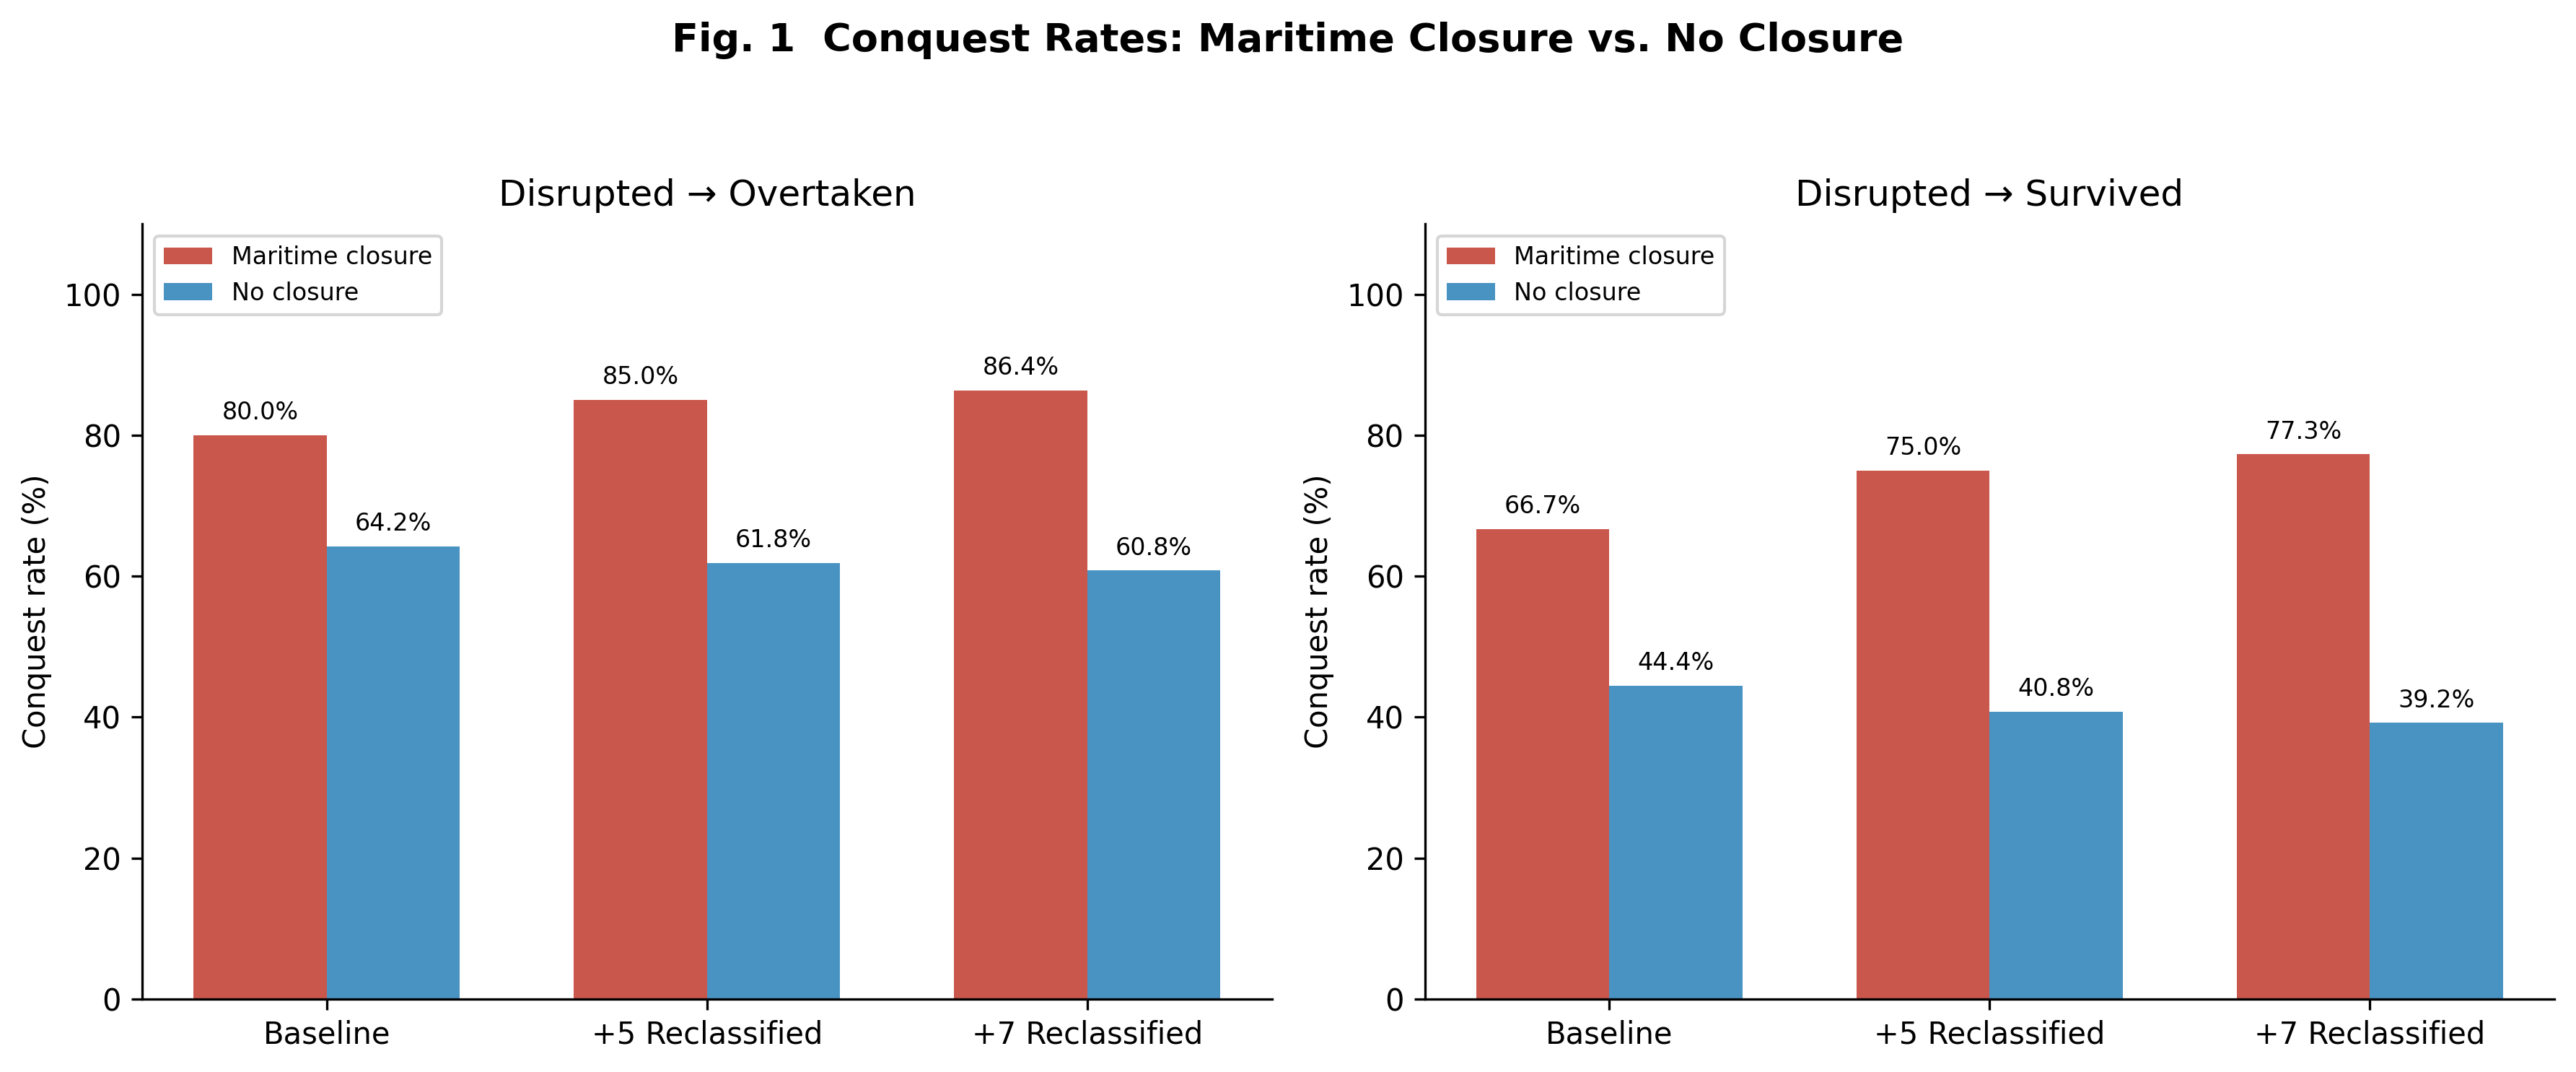
\includegraphics[width=\textwidth]{figures/Fig1.png}
\caption{Conquest rates comparing network closure vs.\ open polities across three reclassification scenarios under both disrupted assignments.}
\label{fig:conquest-rates}
\end{figure}

Figure~\ref{fig:fisher-pvalues} shows how the one-sided Fisher $p$-value changes under the same reclassification sequence.

\begin{figure}[htbp]
\centering
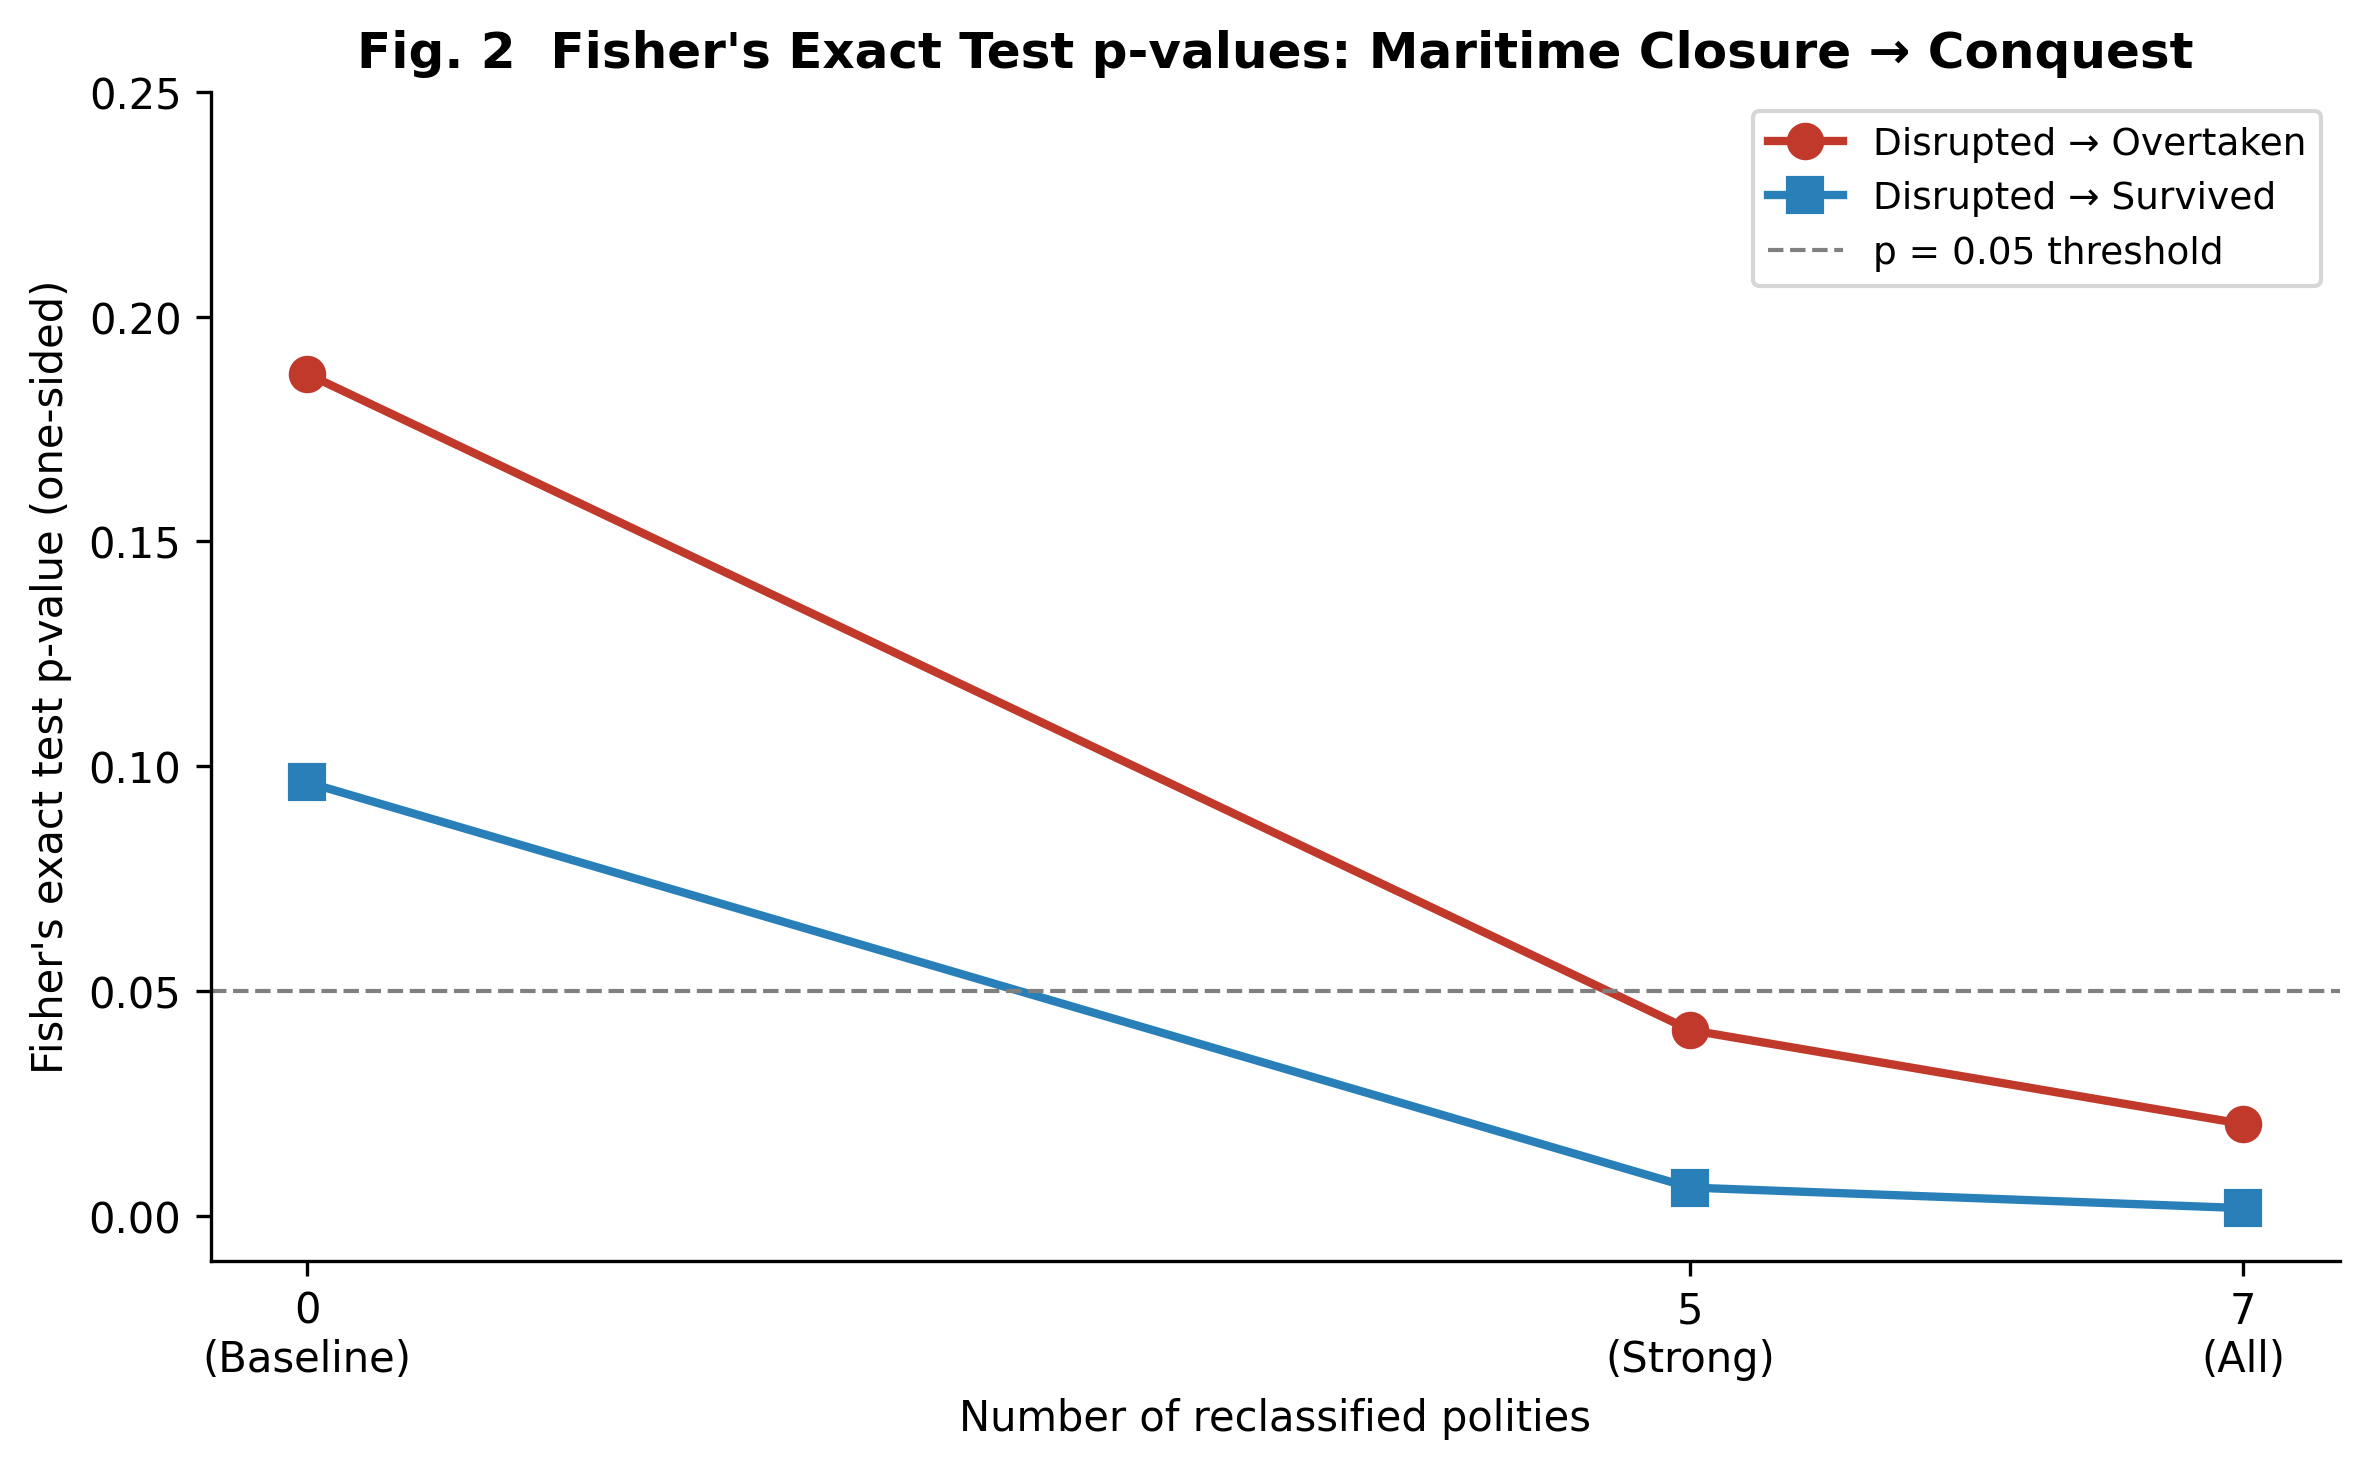
\includegraphics[width=0.85\textwidth]{figures/Fig2.png}
\caption{Fisher's exact test $p$-values for the network closure $\to$ conquest association as polities are progressively reclassified.}
\label{fig:fisher-pvalues}
\end{figure}

\section{Sensitivity Analysis: Technical Network Exclusion}\label{sec:sensitivity}

\subsection{Closure-type disaggregation}\label{sec:sensitivity-dose}

Under the 7-country reclassification, technically excluded polities---those classified as severely disconnected from the dominant exchange networks of their era---have a 100.0\% conquest rate. Policy-based maritime bans, which restricted but did not entirely eliminate external contact, show lower rates (76.9\% under disrupted $\to$ overtaken; 69.2\% under disrupted $\to$ survived). \emph{Sakoku} polities show 100.0\% and 50.0\% rates under the two assignments, reflecting the borderline case of Tokugawa Japan, which maintained a narrow technological conduit (\emph{rangaku}) through Dejima. Bloc-type closures show the lowest conquest rates among closure categories, consistent with the interpretation that bloc membership preserves some technology transfer through alliance-internal channels.

Figure~\ref{fig:closure-types} shows that the category rates are not strictly monotonic: technical exclusion and \emph{sakoku} have the highest rates, maritime bans are intermediate, and bloc closure is lower than the open category. The disaggregation therefore motivates the technology-flow hypothesis but does not independently establish a dose--response relationship.

\begin{figure}[htbp]
\centering
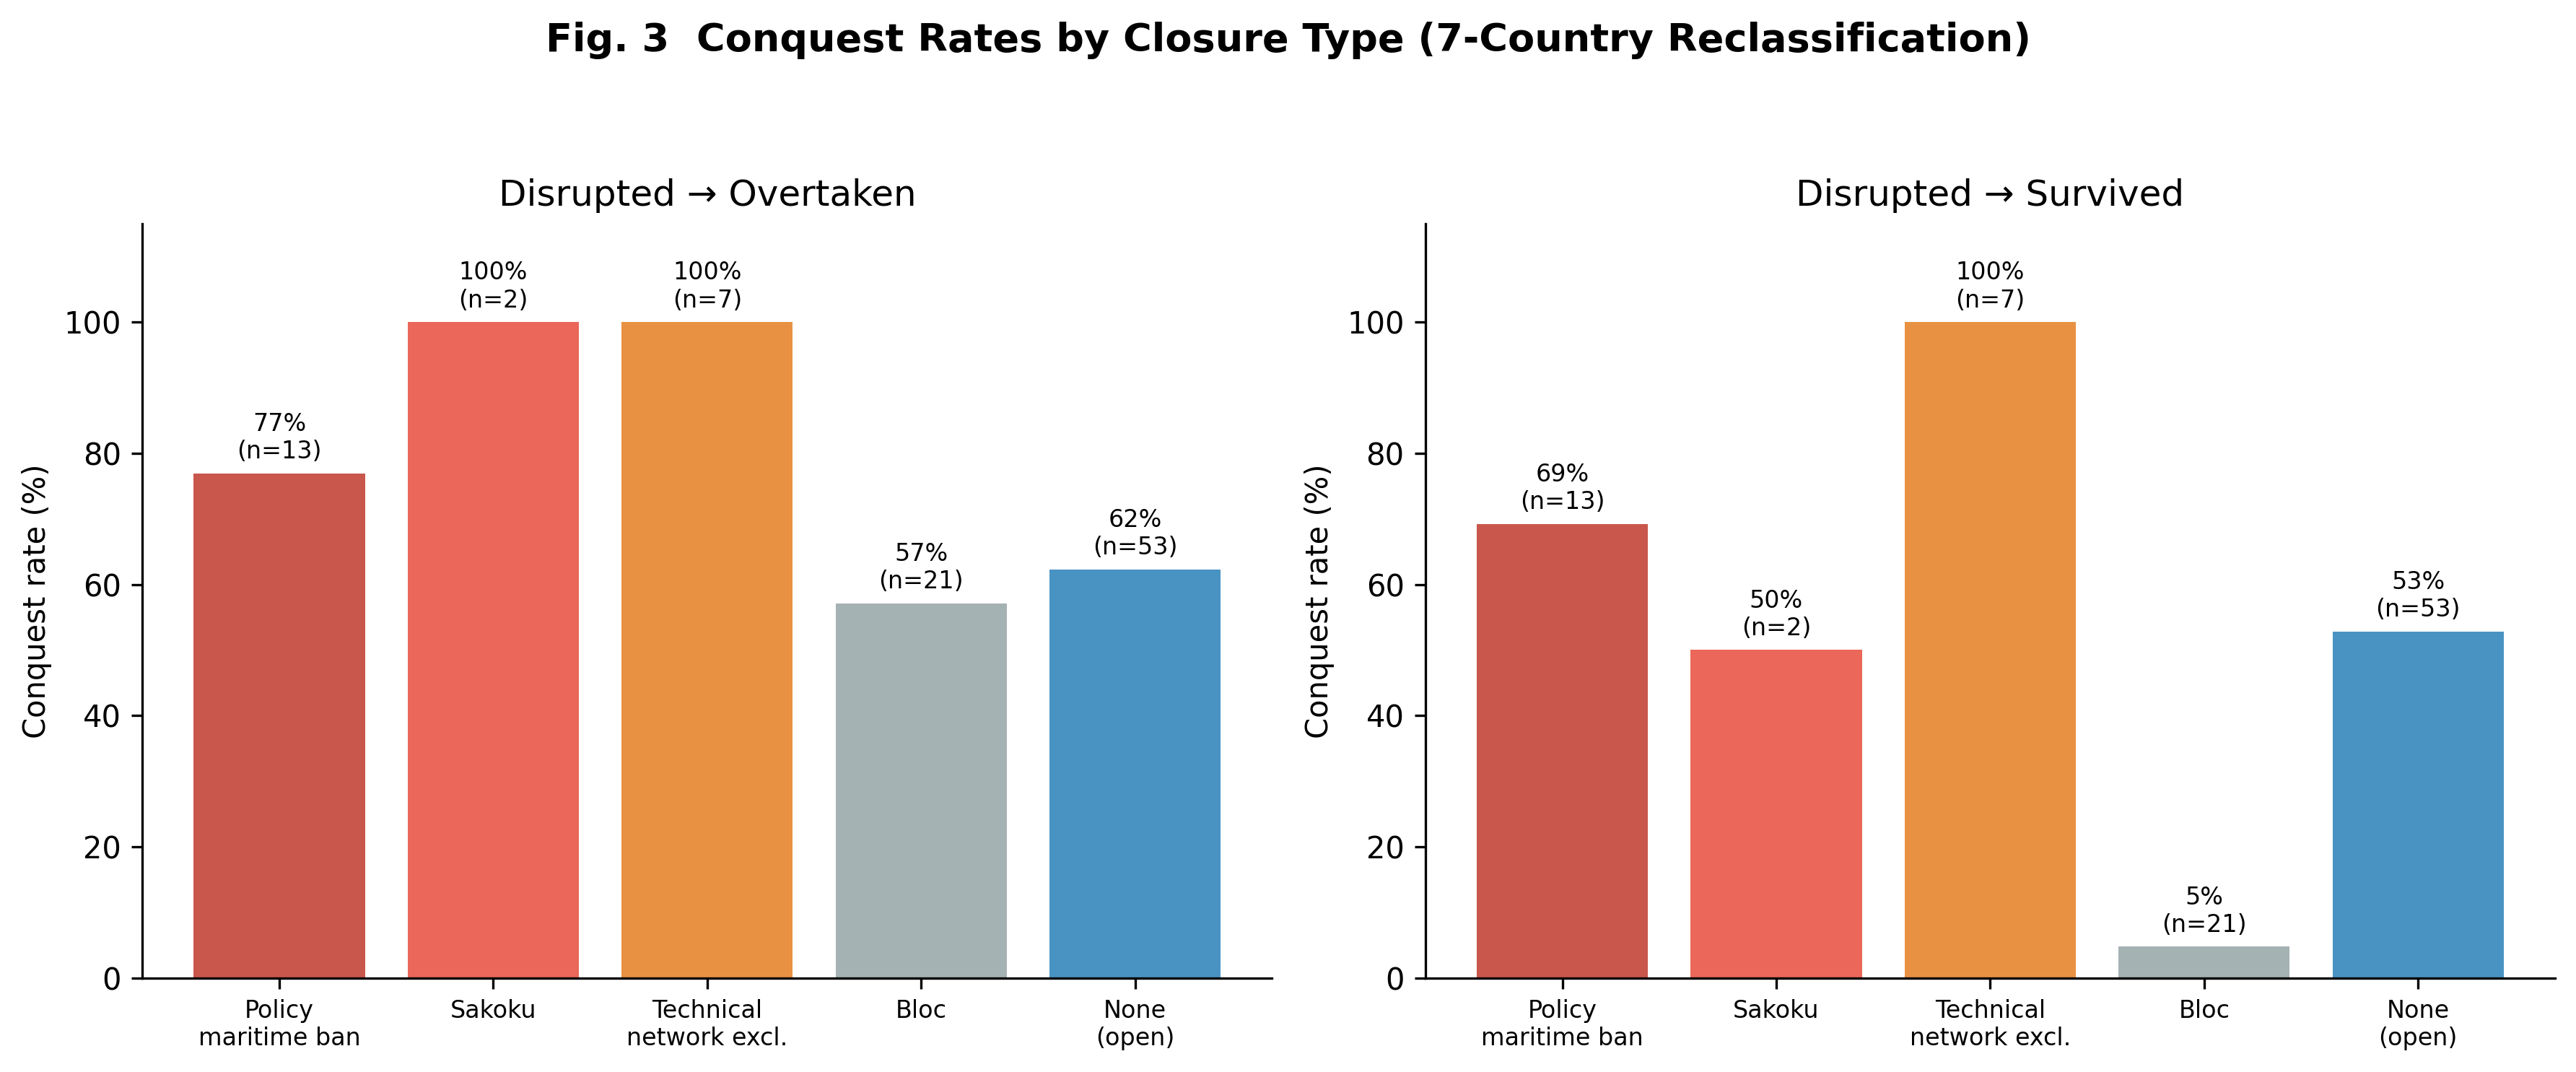
\includegraphics[width=\textwidth]{figures/Fig3.png}
\caption{Conquest rates by closure type under the 7-country reclassification scenario.}
\label{fig:closure-types}
\end{figure}

\subsection{Stability of the stock--flow odds ratio}\label{sec:sensitivity-or}

The stock--flow OR $= 1.774$ is identical across all three reclassification scenarios. This invariance is expected: the reclassification changes the closure-type label but does not alter the stock/flow or outcome coding. Bootstrap resampling (5{,}000 draws) yields a median OR of $1.794$ (95\% CI [0.742, 4.601]), The median is close to the point estimate, but the interval is wide and includes the null.

\subsection{Multivariate regression stability}\label{sec:sensitivity-regression}

Figure~\ref{fig:forest-plot} presents the multivariate logistic regression results under the 7-country reclassification with disrupted $\to$ overtaken. In this specification, external threat ($p = 0.0033$), institutional quality ($p = 0.0074$), and era ($p = 0.0093$) have the smallest p-values. The network closure indicator is not independently significant ($p = 0.8630$) after controlling for these covariates. This pattern is consistent with, but does not identify, an indirect pathway involving technological stagnation, institutional change, and heightened external vulnerability---covariates that the multivariate model already captures.

\begin{figure}[htbp]
\centering
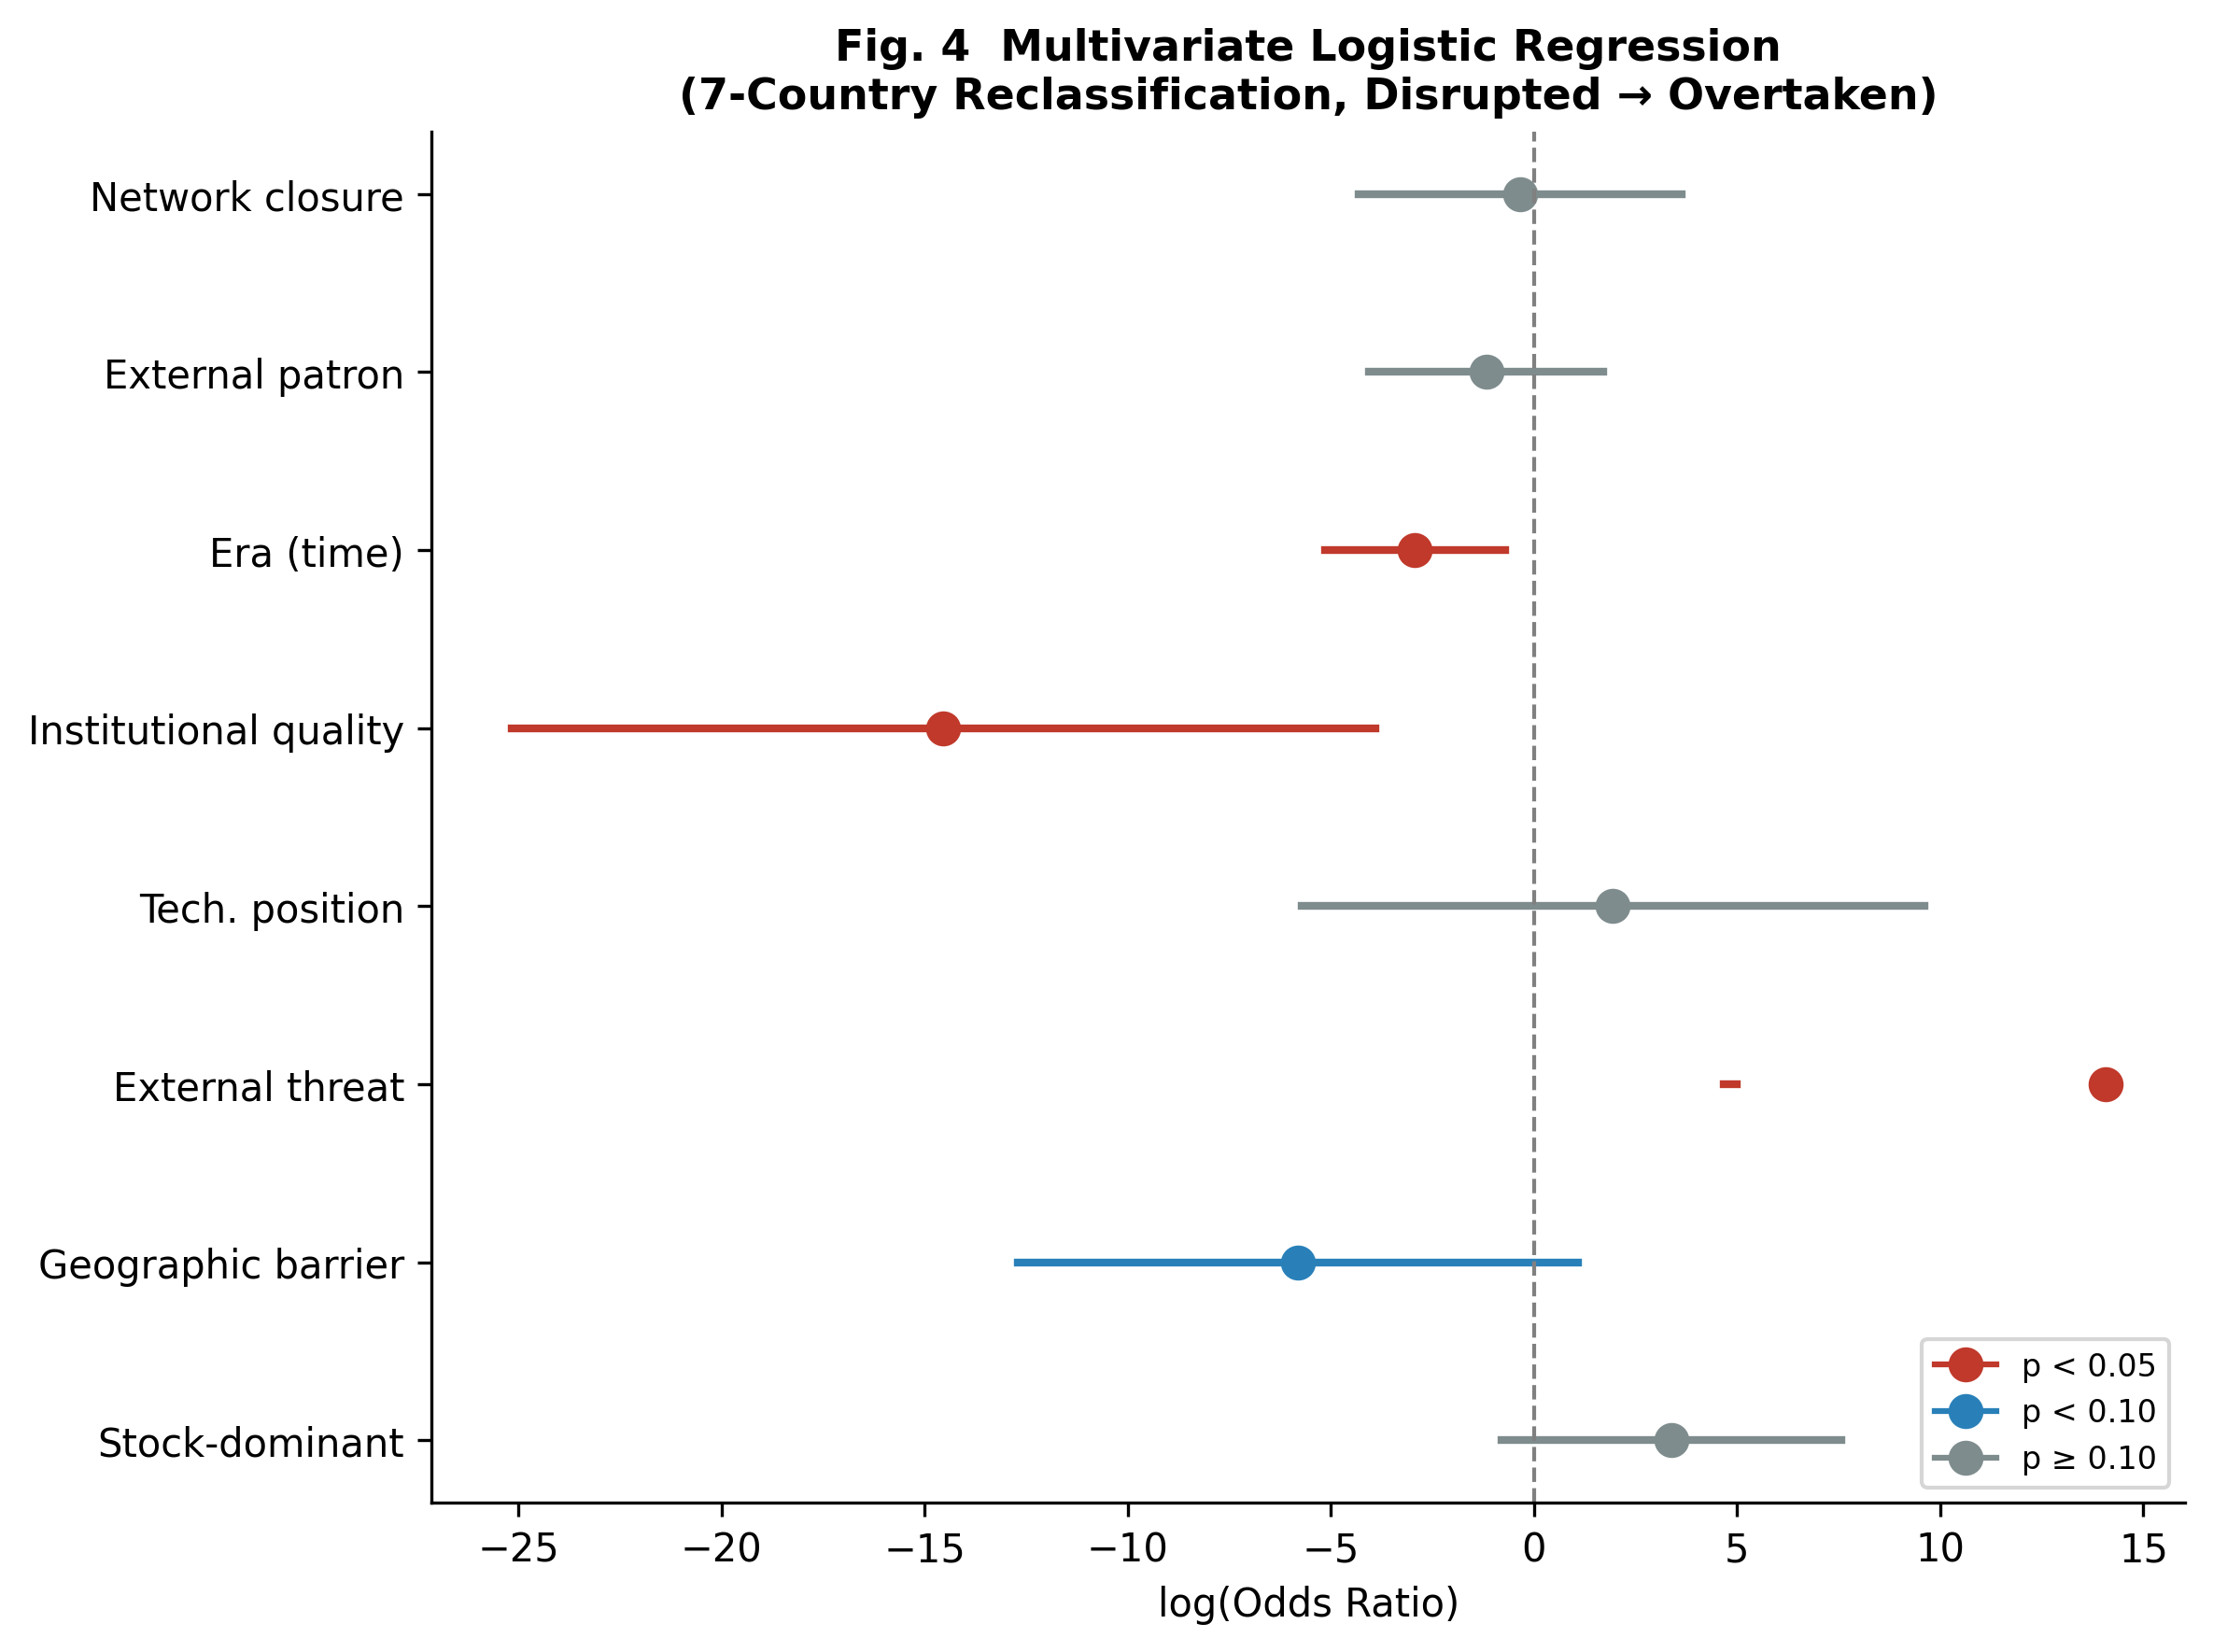
\includegraphics[width=0.9\textwidth]{figures/Fig4.png}
\caption{Forest plot of multivariate logistic regression odds ratios (7-country reclassification, disrupted $\to$ overtaken).}
\label{fig:forest-plot}
\end{figure}

Table~\ref{tab:regression} reports the corresponding coefficients, confidence intervals, and $p$-values.

\begin{table}[htbp]
\caption{Multivariate logistic regression results (7-country reclassification, disrupted $\to$ overtaken). $^{*}$~$p < 0.05$, $^{\dag}$~$p < 0.10$.}
\label{tab:regression}
\begin{tabular*}{\textwidth}{@{\extracolsep\fill}lcccc}
\toprule
Variable & OR & 95\% CI & $p$-value & Sig. \\
\midrule
Stock-dominant & 29.619 & [0.452, 1939.410] & 0.1123 &  \\
Geographic barrier & 0.003 & [0.000, 2.942] & 0.0983 & \dag \\
External threat & 1279858.850 & [106.606, $>10^{6}$] & 0.0033 & * \\
Technological position & 6.973 & [0.003, 14940.014] & 0.6197 &  \\
Institutional quality & 0.000 & [0.000, 0.020] & 0.0074 & * \\
Era (time) & 0.053 & [0.006, 0.486] & 0.0093 & * \\
External patron & 0.309 & [0.017, 5.520] & 0.4247 &  \\
Network closure dummy & 0.705 & [0.013, 37.496] & 0.8630 &  \\
\botrule
\end{tabular*}
\end{table}

\section{Discussion}\label{sec:discussion}

\subsection{The mechanism: technology flow disruption and cumulative divergence}\label{sec:disc-mechanism}

In the post hoc sensitivity analysis, the closure--conquest association changes when technically excluded polities are grouped with deliberately closed ones. This classification sensitivity suggests a pattern relevant to the proposed mechanism. If closure harmed states solely through lost trade revenue or reduced diplomatic leverage, then only deliberate closure---which blocks trade but not necessarily knowledge---should matter. Treating technical exclusion as a more severe disconnection category strengthens the association relative to the policy-only coding, which is consistent with technology flow as a candidate channel.

The closure-type pattern in Figure~\ref{fig:closure-types} provides a descriptive comparison. Technical exclusion (classified as severe disconnection) is associated with a 100.0\% conquest rate. Policy-based maritime bans, which restrict but do not eliminate technology flow, show a 76.9\% rate under the main assignment. The case of Tokugawa Japan is particularly instructive: despite the comprehensive closure of \emph{sakoku}, the Tokugawa regime deliberately maintained a narrow conduit for Western scientific and technical knowledge (\emph{rangaku}) through the Dutch trading post at Dejima. This selective preservation of a technology transfer channel---even within an otherwise closed system---is consistent with its avoidance of conquest. Japan was disrupted by the forced opening of 1853--54 but was not conquered; it reconstituted itself as the Meiji state and rapidly closed the technology gap. Bloc closures, which preserve substantial within-bloc technology sharing, show the lowest rate among closure categories. Because the category rates are not strictly monotonic, this comparison is hypothesis-generating rather than evidence of a dose--response relationship.

The multivariate results provide a descriptive comparison. External threat and institutional quality have the largest conditional associations with conquest, and the network closure indicator loses significance after their inclusion (Table~\ref{tab:regression}, Fig.~\ref{fig:forest-plot}). This is compatible with a technology-gap hypothesis, but does not establish one. One possible sequence is that technological stagnation weakens institutional adaptive capacity and leaves a polity less able to respond to external threats. This proposed ordering is consistent with \citeauthor{AcemogluRobinson2012}'s (\citeyear{AcemogluRobinson2012}) emphasis on institutions as a proximate determinant of national success. Network access is treated here as a possible antecedent for future testing, not as an identified upstream cause. The candidate mediating variables (external threat, institutional quality) absorb the conditional association of the closure variable, but the cross-sectional exploratory design cannot establish direction, mediation, or causation.

\subsection{First contact and a proposed divergence mechanism}\label{sec:disc-firstcontact}

The exploratory results can be read as a quantitative formulation of a long-recognized historical pattern: when civilizations that have developed in isolation encounter a technologically superior civilization, asymmetric outcomes may follow \citep{Diamond1997, DiamondBellwood2003}. Within this selected dataset, 100.0\% of technically excluded cases are coded as conquered. The post hoc classification and non-probability case selection prevent treating that descriptive rate as a general historical estimate.

The hypothesized pathway is cumulative divergence through technology flow disruption. International exchange networks carried not only goods but military techniques, metallurgical innovations, navigational knowledge, and institutional models \citep{Mokyr2002, Pomeranz2000}. Polities connected to these networks could adopt, adapt, and build upon innovations generated elsewhere. Polities with weaker access may have less capacity to do so. Over generations, a technology gap may widen---a process analogous to the long-run consequences of network disruption documented by \citet{Nunn2008}, who showed that regions more heavily affected by the slave trade experienced persistent underdevelopment centuries later. When contact with a more advanced civilization eventually occurred---often through military expansion---an accumulated gap may have contributed to vulnerability. These case narratives motivate the proposed sequence but do not test it.

Policy-closed polities that maintained narrow conduits of technology transfer---Japan's \emph{rangaku} and Qing China's limited Canton trade---suggest a contrast worth testing against more severe disconnection. The present data do not measure residual technology flow or cumulative gaps and therefore cannot determine whether those mechanisms explain the coded outcomes.

This finding has a corollary that is worth stating explicitly. If the critical variable is not closure itself but the residual technology flow that closure permits, then polities that close their borders while deliberately maintaining selective channels for frontier knowledge occupy a qualitatively different position from those that are more severely disconnected. Our dataset contains several instances of such conditional closure. Tokugawa Japan preserved access to Western science through \emph{rangaku} at Dejima and was disrupted but not conquered, reconstituting itself as the Meiji state. Early Qing China maintained the Canton system---a single, tightly controlled port of trade through which some foreign knowledge filtered---and survived the Kangxi--Qianlong era intact. Joseon Korea sustained tributary trade with China, which served as a conduit for Continental knowledge and technology. The Soviet Union, while sealed from the Western bloc, maintained extensive technology sharing within the Eastern bloc and invested heavily in indigenous research institutions. North Korea has preserved a limited technology channel through its relationship with China. (Full details of each polity's closure regime, technology channels, and outcomes are recorded in Supplementary Table~S1.)

The outcomes, however, are mixed. Early Qing China survived, but late Qing China---operating under the same Canton system---was semi-colonized after the Opium Wars. Tokugawa Japan survived as a political entity, but Joseon Korea, despite its Chinese conduit, was annexed by Japan in 1910. The Soviet Union collapsed internally despite its bloc-level technology sharing, while North Korea has persisted under extreme isolation with minimal Chinese patronage. These divergent outcomes suggest that the mere existence of a selective channel does not guarantee survival; unmeasured factors---the breadth and relevance of the knowledge flowing through the channel, the domestic capacity to absorb and adapt that knowledge, the pace of change at the technological frontier, and institutional dynamics that our dataset does not capture---likely condition the effectiveness of conditional closure. The policy question, then, is not binary (open or closed) but conditional, and the conditions under which selective channels suffice to prevent a large technology gap remain an open and consequential problem for future research. Readers interested in tracing these cases in detail are referred to Supplementary Table~S1, which documents the specific turning-point events and outcomes for all 96 polities in the dataset.

\subsection{Beyond geographic isolation: technological access exclusion in the modern era}\label{sec:disc-modern}

If the mechanism we identify is technology flow disruption rather than network closure per se, then the pattern should generalize beyond the age of sail. Each era has its own dominant technological platform---the infrastructure through which frontier knowledge diffuses across states. In antiquity, it was the Mediterranean trade routes and Silk Road caravans. In the early modern period, it was oceanic shipping. In the industrial age, it was railroad-linked factory systems and colonial supply chains. In the twentieth century, it was aerospace and nuclear technology networks.

Today, the dominant platform has shifted again. The critical networks are semiconductor supply chains, artificial intelligence research ecosystems, and advanced robotics and automation infrastructure \citep{AcemogluRestrepo2020, CominMestieri2018}. \citet{CominEasterlyGong2010} show that technology adoption levels in 1000~BC predict income differences today, while \citet{AcemogluJohnsonRobinson2002} demonstrate that colonial-era institutional reversals reshaped global inequality---both consistent with the view that early technological access has persistent, cumulative consequences. Global shipping and communication networks have reduced, but not eliminated, geographic barriers to exchange. A further form of structural exclusion may arise when states are cut off from the technological frontier not by mountains and oceans but by export controls on advanced semiconductors, by the concentration of AI training infrastructure in a handful of countries, or by the institutional and human-capital barriers that prevent participation in cutting-edge research networks.

An exploratory analogy can be drawn to contemporary states excluded from advanced semiconductor fabrication or AI model development, which may face a widening technology gap. If the gap grows large enough, the eventual `first contact'---whether military, economic, or geopolitical---could produce asymmetric outcomes. Whether the historical coding captures a comparable process is an empirical question for future data.

We stress that this extrapolation is speculative and cannot be tested within our historical dataset. The contemporary world differs from the premodern era in ways that may attenuate or amplify the mechanism: nuclear deterrence, international institutions, and the speed of modern communication all introduce novel dynamics. The post hoc association in the selected cases provides a provisional framework for thinking about which dimensions of modern technological access may be most consequential.

\subsection{Stability of the stock--flow framework and the question of resource-base transitions}\label{sec:disc-stockflow}

The stock--flow OR (1.774) is unchanged across the reclassification scenarios because those scenarios alter closure labels but not stock/flow or outcome coding. The stock--flow and closure comparisons should therefore be interpreted as separate exploratory descriptions rather than as evidence of distinct causal dimensions.

Crossing these two dimensions yields a four-cell classification whose conquest rates are reported in Table~\ref{tab:stockflow-closure}. Flow-oriented polities without closure show the lowest conquest rate (57.4\%, $n = 47$). Stock-oriented polities without closure show a moderately elevated rate (66.7\%, $n = 27$). Stock-oriented polities with closure show a markedly higher rate (83.3\%, $n = 18$). Flow-oriented polities with closure---a small cell ($n = 4$)---show a 100.0\% conquest rate. The contrast between the highest- and lowest-risk cells (stock + closed vs.\ flow + open) yields an odds ratio of 3.70 (one-sided Fisher exact $p = 0.045$). Within stock-oriented polities, the effect of closure corresponds to an OR of 2.50 ($p = 0.187$). Within flow-oriented polities, the effect of closure yields an OR of $\infty$ ($p = 0.126$), though the cell size ($n = 4$) precludes reliable inference.

\begin{table}[htbp]
\caption{Conquest rates by resource-base orientation and closure status (7-country reclassification, disrupted $=$ conquered).}
\label{tab:stockflow-closure}
\begin{tabular*}{\textwidth}{@{\extracolsep\fill}lcccc}
\toprule
 & Conquered & Survived & $n$ & Rate \\
\midrule
Stock + closed & 15 & 3 & 18 & 83.3\% \\
Stock + open & 18 & 9 & 27 & 66.7\% \\
Flow + closed & 4 & 0 & 4 & 100.0\% \\
Flow + open & 27 & 20 & 47 & 57.4\% \\
\botrule
\end{tabular*}
\footnotetext{Fisher exact tests (one-sided): stock + closed vs.\ flow + open, OR $= 3.70$, $p = 0.045$; within stock, closed vs.\ open, OR $= 2.50$, $p = 0.187$; within flow, closed vs.\ open, OR $= \infty$, $p = 0.126$.}
\end{table}

The pattern is consistent with the hypothesis that stock-orientation and network exclusion compound each other's risk, though the small cell sizes---particularly for flow + closed ($n = 4$)---warrant caution. The stock + closed combination is the only cell to reach a statistically significant difference from the baseline flow + open cell at conventional levels. Notably, 3 stock-oriented polities with closure survived despite their high-risk classification; their individual characteristics---including specific closure regimes, technology channels maintained, and the historical circumstances of their survival---are documented in Supplementary Table~S1.

An implication worth noting is that the stock--flow distinction is not permanently fixed for any given state. Polities can transition from flow-oriented to stock-oriented resource bases---or vice versa---as economic structures, demographic conditions, and institutional incentives evolve. A state that was historically flow-oriented (trade-dependent, outward-looking, innovation-absorbing) but that gradually shifts toward reliance on accumulated domestic assets---physical capital, territorial resources, existing institutional infrastructure---moves into the higher-risk stock category. If such a transition coincides with reduced engagement in the dominant technological network of the era, the compounding of stock-orientation and network exclusion could amplify vulnerability. Our dataset cannot test this dynamic directly, as polities are coded at a single point in time, but the theoretical interaction between resource-base transition and network access merits further investigation.

\subsection{Limitations}\label{sec:disc-limitations}

Several limitations warrant acknowledgment. First, the coding of historical polities inevitably involves subjective judgment, particularly for the stock/flow classification and the identification of technical exclusion candidates. The tiered approach (strong vs.\ moderate candidates) and the six-scenario sensitivity design partially address this, but cannot eliminate it. Second, the sample size ($N = 96$) constrains the power of the multivariate analyses; wide confidence intervals for some regression coefficients reflect this constraint. Third, the dataset treats polities as independent observations, though historical interconnections (e.g., sequential Chinese dynasties sharing institutional continuity) may introduce non-independence. Fourth, the `disrupted' category introduces a classification ambiguity that the dual-assignment design addresses but cannot fully resolve. Fifth, the forward-looking extension to modern technological exclusion is necessarily speculative, as the mechanisms operating in a nuclear-armed, institutionally dense modern world may differ qualitatively from those in premodern eras.

\section{Conclusion}\label{sec:conclusion}

Within this AI-assisted exploratory dataset, a post hoc reclassification of 7 technically excluded polities---those coded as disconnected from the dominant exchange networks of their era by geography and technology rather than by policy---changes the one-sided Fisher exact p-value to 0.020, while the core stock--flow odds ratio remains unchanged (OR $= 1.774$). The 100.0\% conquest rate among technically excluded polities, the closure-type comparison, and the absorption of the closure effect by external threat and institutional quality in multivariate models are consistent with, but do not establish, a proposed mechanism in which disruption of technology flow leads to cumulative divergence from the technological frontier.

The broader implication is that this mechanism is not specific to any single network form. In every era, there exists a dominant network through which frontier technologies diffuse. Polities excluded from that network---whether by oceans, mountains, policy, or, in the contemporary period, by semiconductor export controls and AI infrastructure concentration---may warrant comparison with historical patterns of cumulative divergence. The exploratory comparison does not establish that modern technological restrictions will produce the same outcomes. The converse question suggested by the Tokugawa precedent is whether a state that recognizes the risk of network exclusion can, through deliberate maintenance of selective technology channels, reduce divergence while restricting broader engagement with the outside world.

\section*{Statements and Declarations}

\subsection*{Funding}
[To be completed by author]

\subsection*{Competing Interests}
[To be confirmed by author]

\subsection*{Author Contributions (CRediT)}
[To be completed by author]

\subsection*{Data Availability}
The complete dataset and analysis code are available at \url{https://github.com/bougtoir/beyond-gdp-national-power}. Supplementary Table~S1 provides the full dataset of 96 polities with all coded variables.

\subsection*{Declaration of Generative AI and AI-Assisted Technologies in the Manuscript Preparation Process}
During the preparation of this work, the author used Devin (Cognition AI) to support code execution, dataset documentation, source auditing, and drafting and editing. The author reviewed and edited the content as needed and takes full responsibility for the content of the published article. [Author confirmation required before submission.]

\subsection*{JEL Classification}
N40, N70, F50, O33, C25

\bibliography{references}

\end{document}